\chapter{Soluci\'on de sistemas no lineales}

En este cap\'itulo veremos el modo de soluci\'on de los sistemas no lineales, que son aquellos en los que por lo menos una de sus ecuaciones no es lineal(hay un grado mayor que uno), o bien hay funciones compuestas.\\
\begin{center}
Un ejemplo de uso es en los circuitod de corriente alterna, as\'i como en las redes hidr\'aulicas
\begin{center}
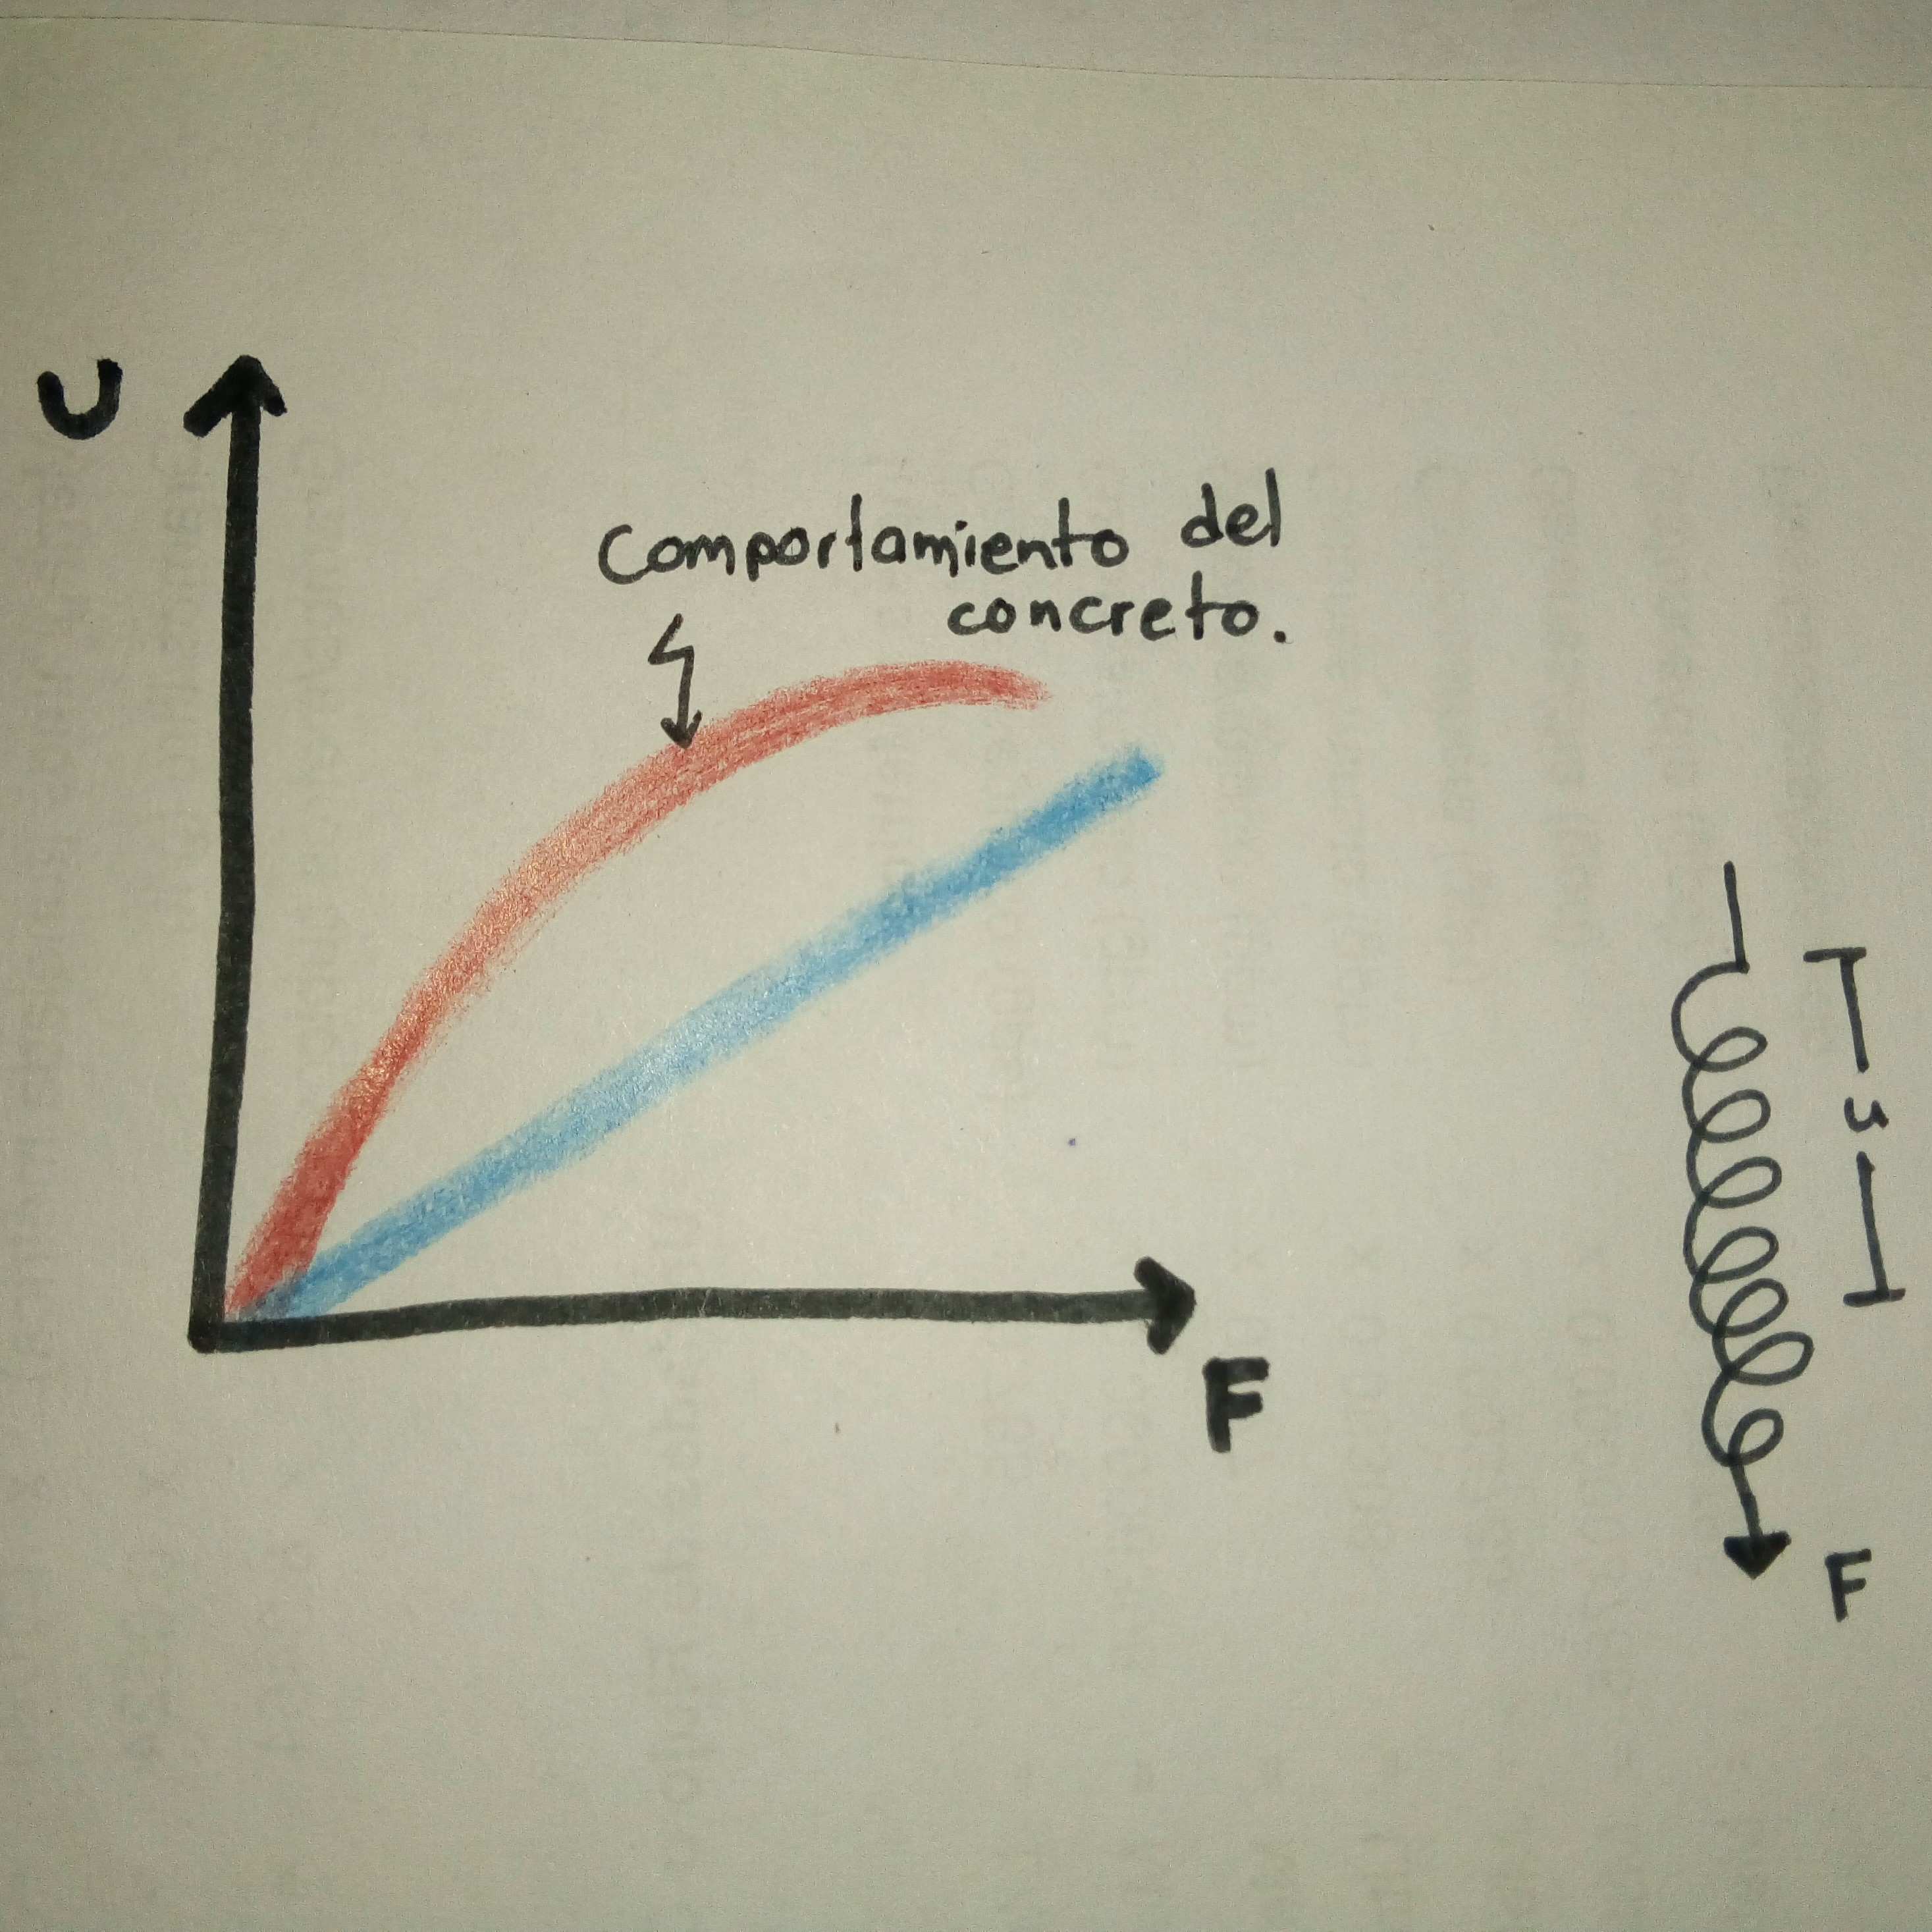
\includegraphics[scale=.05]{imagenes/13.jpg}
\end{center}
\end{center}
%ilustraciones de graficas y resorte%
$u=kF$\\
$u=k(u,F)$\\
\begin{displaymath}
f_1(x_1,x_2,x_3,x_4,\cdots, x_n)=0
\end{displaymath}
\begin{displaymath}
f_2(x_1,x_2,x_3,x_4,\cdots, x_n)=0
\end{displaymath}
\begin{displaymath}
f_3(x_1,x_2,x_3,x_4,\cdots, x_n)=0
\end{displaymath}
\begin{center}
$\vdots$
\end{center}
\begin{displaymath}
f_n(x_1,x_2,x_3,x_4,\cdots, x_n)=0
\end{displaymath}
\begin{displaymath}
F=\begin{bmatrix}
f_1(x)\\
f_2(x)\\
f_3(x)\\
\vdots \\
f_n(x)
\end{bmatrix}; \qquad x=\begin{bmatrix}
x_1\\
x_2\\
x_3\\
\vdots \\
x_n
\end{bmatrix}
\end{displaymath}
$F(x)=0; \qquad f(x)=0$\\
\begin{displaymath}
F(x^{k+1})=F(x^k)+F'(x^k)(x^{k+1}-x^k)\mid +F'(x^k)\frac{(x^{k+1}-x^k)^2}{2!}
\end{displaymath}
$0=F(x^k)+F'(x^k)(x^{k+1}-x^k)$\\
\begin{center}
Matriz Jacobiana del sistema
\end{center}
\begin{displaymath}
F'(x)=\begin{bmatrix}
\nabla f_1(x)^T \\
\nabla f_2(x)^T \\
\nabla f_3(x)^T \\
\vdots \\
\nabla f_n(x)^T
\end{bmatrix}=\begin{bmatrix}
\frac{\delta f_1}{\delta x_1} & \frac{\delta f_1}{\delta x_2} & \frac{\delta f_1}{\delta x_3} & \cdots & \frac{\delta f_1}{\delta x_n} \\
\frac{\delta f_2}{\delta x_1} & \frac{\delta f_2}{\delta x_2} & \frac{\delta f_2}{\delta x_3} & \cdots & \frac{\delta f_2}{\delta x_n} \\
\vdots & \vdots & \vdots & \ddots & \vdots \\ \frac{\delta f_n}{\delta x_1} & \frac{\delta f_n}{\delta x_2} & \frac{\delta f_n}{\delta x_3} & \cdots & \frac{\delta f_n}{\delta x_n} \\
\end{bmatrix}
\end{displaymath}
$s^k=x^{k+1}-x^k$\\
\begin{displaymath}
F'(x^k)(s^k)=-F(x^k)
\end{displaymath}
Se resuelve el sistema para obtener posteriormente el valor de $x^{k+1}$



%--------------------------------------%

\chapter{Derivadas num\'ericas parciales}
En el primer cap\'itulo hablamos de las derivadas num\'ericas, que hacen referencia a la derivaci\'on respecto a una sola varible. Habr\'a ocasiones en las que la soluc\'on de sistemas deber\'a ser dada por derivadas parciales, ya que los sistemas manejan m\'as de una variable, lo que hace necesario conocer acerca de esto.
%Algoritmo%
Dado $f(x,y)$
\begin{displaymath}
\frac{\delta f}{\delta x}=\lim_{\Delta x \to 0} \frac{f(x+\Delta x, y)-f(x,y)}{\Delta x}
\end{displaymath}
\begin{displaymath}
\frac{\delta f}{\delta y}=\lim_{\Delta y \to 0} \frac{f(x, y\Delta y)-f(x,y)}{\Delta y}
\end{displaymath}
\begin{displaymath}
\frac{\delta f}{\delta x}=\frac{f(x+h, y)-f(x,y)}{h} \qquad ; \qquad \frac{\delta f}{\delta y}=\frac{f(x, y+h)-f(x,y)}{h}
\end{displaymath}
\begin{displaymath}
\frac{\delta f}{\delta x_j}=\frac{f(x_1, x_2, \cdots , x_j+h, \cdots , x_n)-f(x_1,x_2,x_3, \cdots ,x_n)}{h}
\end{displaymath}
\begin{displaymath}
[F'(x)]_{ij}=\frac{f_j(x_1,x_2,x_j+h,\cdots ,x_n)-f_i(x_1, x_2, x_3,\cdots ,x_n)}{h}
\end{displaymath}
%--Hacer un ejemplo--%